

\tikzset{every picture/.style={line width=0.75pt}} %set default line width to 0.75pt

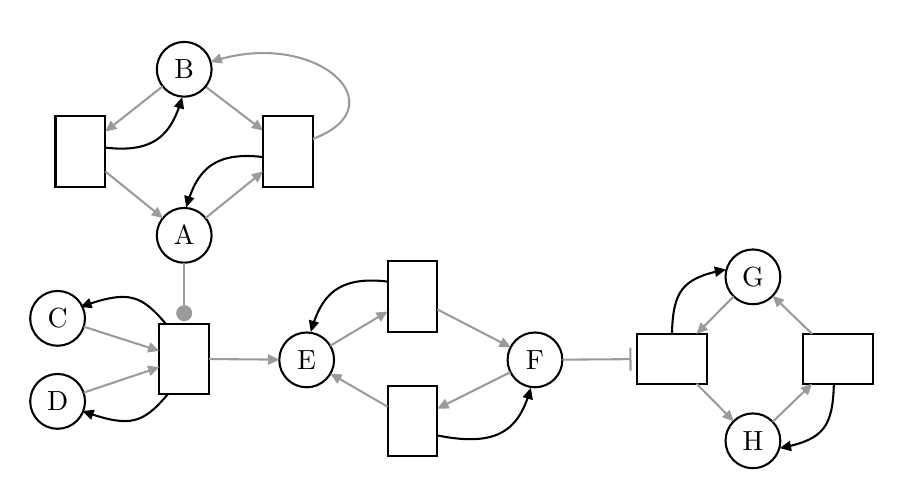
\begin{tikzpicture}[x=0.75pt,y=0.75pt,yscale=-1,xscale=1]
%uncomment if require: \path (0,300); %set diagram left start at 0, and has height of 300

%Straight Lines [id:da5537401684788057]
\draw [color={rgb, 255:red, 155; green, 155; blue, 155 }  ,draw opacity=1 ]   (100,56) -- (135.62,83.18) ;
\draw [shift={(138,85)}, rotate = 217.35] [fill={rgb, 255:red, 155; green, 155; blue, 155 }  ,fill opacity=1 ][line width=0.08]  [draw opacity=0] (5.36,-2.57) -- (0,0) -- (5.36,2.57) -- cycle    ;
%Curve Lines [id:da4219617780524596]
\draw    (150,100) .. controls (116.22,91.94) and (107.13,102.73) .. (101.81,119.33) ;
\draw [shift={(101,122)}, rotate = 286.15999999999997] [fill={rgb, 255:red, 0; green, 0; blue, 0 }  ][line width=0.08]  [draw opacity=0] (5.36,-2.57) -- (0,0) -- (5.36,2.57) -- cycle    ;
%Curve Lines [id:da19935471916041347]
\draw    (50,91) .. controls (83.78,99.06) and (92.87,88.27) .. (98.19,71.67) ;
\draw [shift={(99,69)}, rotate = 466.16] [fill={rgb, 255:red, 0; green, 0; blue, 0 }  ][line width=0.08]  [draw opacity=0] (5.36,-2.57) -- (0,0) -- (5.36,2.57) -- cycle    ;
%Curve Lines [id:da7407078847752033]
\draw    (91,178) .. controls (79.33,164.1) and (72.96,162.07) .. (52.62,169.08) ;
\draw [shift={(50,170)}, rotate = 340.2] [fill={rgb, 255:red, 0; green, 0; blue, 0 }  ][line width=0.08]  [draw opacity=0] (5.36,-2.57) -- (0,0) -- (5.36,2.57) -- cycle    ;
%Curve Lines [id:da6312464386805752]
\draw    (92,212.15) .. controls (80.33,226.05) and (73.96,228.08) .. (53.62,221.08) ;
\draw [shift={(51,220.15)}, rotate = 379.8] [fill={rgb, 255:red, 0; green, 0; blue, 0 }  ][line width=0.08]  [draw opacity=0] (5.36,-2.57) -- (0,0) -- (5.36,2.57) -- cycle    ;
%Curve Lines [id:da6967297725973456]
\draw    (335,183) .. controls (335.46,162.49) and (340.04,156.46) .. (358.32,152.54) ;
\draw [shift={(361,152)}, rotate = 529.1800000000001] [fill={rgb, 255:red, 0; green, 0; blue, 0 }  ][line width=0.08]  [draw opacity=0] (5.36,-2.57) -- (0,0) -- (5.36,2.57) -- cycle    ;
%Curve Lines [id:da9565492179833825]
\draw    (413,207) .. controls (412.54,227.51) and (407.96,233.54) .. (389.68,237.46) ;
\draw [shift={(387,238)}, rotate = 349.18] [fill={rgb, 255:red, 0; green, 0; blue, 0 }  ][line width=0.08]  [draw opacity=0] (5.36,-2.57) -- (0,0) -- (5.36,2.57) -- cycle    ;
%Curve Lines [id:da778026018839471]
\draw    (210,160) .. controls (176.22,151.94) and (167.13,162.73) .. (161.81,179.33) ;
\draw [shift={(161,182)}, rotate = 286.15999999999997] [fill={rgb, 255:red, 0; green, 0; blue, 0 }  ][line width=0.08]  [draw opacity=0] (5.36,-2.57) -- (0,0) -- (5.36,2.57) -- cycle    ;
%Curve Lines [id:da16091612307930925]
\draw    (218,231) .. controls (251.78,239.06) and (260.87,228.27) .. (266.19,211.67) ;
\draw [shift={(267,209)}, rotate = 466.16] [fill={rgb, 255:red, 0; green, 0; blue, 0 }  ][line width=0.08]  [draw opacity=0] (5.36,-2.57) -- (0,0) -- (5.36,2.57) -- cycle    ;

% Text Node
\draw  [fill={rgb, 255:red, 255; green, 255; blue, 255 }  ,fill opacity=1 ]  (38,78) -- (62,78) -- (62,112) -- (38,112) -- cycle  ;
\draw (50,95) node   [align=left] {\begin{minipage}[lt]{13.600000000000001pt}\setlength\topsep{0pt}
\begin{center}
\end{center}

\end{minipage}};
% Text Node
\draw  [fill={rgb, 255:red, 255; green, 255; blue, 255 }  ,fill opacity=1 ]  (100, 55.5) circle [x radius= 13.2, y radius= 13.2]   ;
\draw (100,55.5) node   [align=left] {\begin{minipage}[lt]{14.96pt}\setlength\topsep{0pt}
\begin{center}
\SF{B}
\end{center}

\end{minipage}};
% Text Node
\draw  [fill={rgb, 255:red, 255; green, 255; blue, 255 }  ,fill opacity=1 ]  (138,78) -- (162,78) -- (162,112) -- (138,112) -- cycle  ;
\draw (150,95) node   [align=left] {\begin{minipage}[lt]{13.600000000000001pt}\setlength\topsep{0pt}
\begin{center}
\end{center}

\end{minipage}};
% Text Node
\draw  [fill={rgb, 255:red, 255; green, 255; blue, 255 }  ,fill opacity=1 ]  (100, 135.5) circle [x radius= 13.2, y radius= 13.2]   ;
\draw (100,135.5) node   [align=left] {\begin{minipage}[lt]{14.96pt}\setlength\topsep{0pt}
\begin{center}
\SF{A}
\end{center}

\end{minipage}};
% Text Node
\draw  [fill={rgb, 255:red, 255; green, 255; blue, 255 }  ,fill opacity=1 ]  (39, 175.5) circle [x radius= 13.2, y radius= 13.2]   ;
\draw (39,175.5) node   [align=left] {\begin{minipage}[lt]{14.96pt}\setlength\topsep{0pt}
\begin{center}
\SF{C}
\end{center}

\end{minipage}};
% Text Node
\draw  [fill={rgb, 255:red, 255; green, 255; blue, 255 }  ,fill opacity=1 ]  (39, 215.5) circle [x radius= 13.2, y radius= 13.2]   ;
\draw (39,215.5) node   [align=left] {\begin{minipage}[lt]{14.96pt}\setlength\topsep{0pt}
\begin{center}
\SF{D}
\end{center}

\end{minipage}};
% Text Node
\draw  [fill={rgb, 255:red, 255; green, 255; blue, 255 }  ,fill opacity=1 ]  (88,178) -- (112,178) -- (112,212) -- (88,212) -- cycle  ;
\draw (100,195) node   [align=left] {\begin{minipage}[lt]{13.600000000000001pt}\setlength\topsep{0pt}
\begin{center}
\end{center}

\end{minipage}};
% Text Node
\draw  [fill={rgb, 255:red, 255; green, 255; blue, 255 }  ,fill opacity=1 ]  (159, 195.5) circle [x radius= 13.2, y radius= 13.2]   ;
\draw (159,195.5) node   [align=left] {\begin{minipage}[lt]{14.96pt}\setlength\topsep{0pt}
\begin{center}
\SF{E}
\end{center}

\end{minipage}};
% Text Node
\draw  [fill={rgb, 255:red, 255; green, 255; blue, 255 }  ,fill opacity=1 ]  (198,148) -- (222,148) -- (222,182) -- (198,182) -- cycle  ;
\draw (210,165) node   [align=left] {\begin{minipage}[lt]{13.600000000000001pt}\setlength\topsep{0pt}
\begin{center}
\end{center}

\end{minipage}};
% Text Node
\draw  [fill={rgb, 255:red, 255; green, 255; blue, 255 }  ,fill opacity=1 ]  (198,208) -- (222,208) -- (222,242) -- (198,242) -- cycle  ;
\draw (210,225) node   [align=left] {\begin{minipage}[lt]{13.600000000000001pt}\setlength\topsep{0pt}
\begin{center}
\end{center}

\end{minipage}};
% Text Node
\draw  [fill={rgb, 255:red, 255; green, 255; blue, 255 }  ,fill opacity=1 ]  (269, 195.5) circle [x radius= 13.2, y radius= 13.2]   ;
\draw (269,195.5) node   [align=left] {\begin{minipage}[lt]{14.96pt}\setlength\topsep{0pt}
\begin{center}
\SF{F}
\end{center}

\end{minipage}};
% Text Node
\draw  [fill={rgb, 255:red, 255; green, 255; blue, 255 }  ,fill opacity=1 ]  (318,183) -- (352,183) -- (352,207) -- (318,207) -- cycle  ;
\draw (335,195) node   [align=left] {\begin{minipage}[lt]{20.400000000000002pt}\setlength\topsep{0pt}
\begin{center}
\end{center}

\end{minipage}};
% Text Node
\draw  [fill={rgb, 255:red, 255; green, 255; blue, 255 }  ,fill opacity=1 ]  (398,183) -- (432,183) -- (432,207) -- (398,207) -- cycle  ;
\draw (415,195) node   [align=left] {\begin{minipage}[lt]{20.400000000000002pt}\setlength\topsep{0pt}
\begin{center}
\end{center}

\end{minipage}};
% Text Node
\draw  [fill={rgb, 255:red, 255; green, 255; blue, 255 }  ,fill opacity=1 ]  (374, 155.5) circle [x radius= 13.2, y radius= 13.2]   ;
\draw (374,155.5) node   [align=left] {\begin{minipage}[lt]{14.96pt}\setlength\topsep{0pt}
\begin{center}
\SF{G}
\end{center}

\end{minipage}};
% Text Node
\draw  [fill={rgb, 255:red, 255; green, 255; blue, 255 }  ,fill opacity=1 ]  (374, 234.5) circle [x radius= 13.2, y radius= 13.2]   ;
\draw (374,234.5) node   [align=left] {\begin{minipage}[lt]{14.96pt}\setlength\topsep{0pt}
\begin{center}
\SF{H}
\end{center}

\end{minipage}};
% Connection
\draw [color={rgb, 255:red, 155; green, 155; blue, 155 }  ,draw opacity=1 ]   (89.64,63.68) -- (64.35,83.66) ;
\draw [shift={(62,85.52)}, rotate = 321.69] [fill={rgb, 255:red, 155; green, 155; blue, 155 }  ,fill opacity=1 ][line width=0.08]  [draw opacity=0] (5.36,-2.57) -- (0,0) -- (5.36,2.57) -- cycle    ;
% Connection
\draw [color={rgb, 255:red, 155; green, 155; blue, 155 }  ,draw opacity=1 ]   (62,104.72) -- (87.41,125.3) ;
\draw [shift={(89.74,127.19)}, rotate = 219.01] [fill={rgb, 255:red, 155; green, 155; blue, 155 }  ,fill opacity=1 ][line width=0.08]  [draw opacity=0] (5.36,-2.57) -- (0,0) -- (5.36,2.57) -- cycle    ;
% Connection
\draw [color={rgb, 255:red, 155; green, 155; blue, 155 }  ,draw opacity=1 ]   (110.26,127.19) -- (135.67,106.61) ;
\draw [shift={(138,104.72)}, rotate = 500.99] [fill={rgb, 255:red, 155; green, 155; blue, 155 }  ,fill opacity=1 ][line width=0.08]  [draw opacity=0] (5.36,-2.57) -- (0,0) -- (5.36,2.57) -- cycle    ;
% Connection
\draw [color={rgb, 255:red, 155; green, 155; blue, 155 }  ,draw opacity=1 ]   (100,148.7) -- (100,173) ;
\draw [shift={(100,173)}, rotate = 90] [color={rgb, 255:red, 155; green, 155; blue, 155 }  ,draw opacity=1 ][fill={rgb, 255:red, 155; green, 155; blue, 155 }  ,fill opacity=1 ][line width=0.75]      (0, 0) circle [x radius= 3.35, y radius= 3.35]   ;
% Connection
\draw [color={rgb, 255:red, 155; green, 155; blue, 155 }  ,draw opacity=1 ]   (162,89.03) .. controls (203.8,73.44) and (164.07,35.95) .. (114.99,51.28) ;
\draw [shift={(112.74,52.02)}, rotate = 341.03] [fill={rgb, 255:red, 155; green, 155; blue, 155 }  ,fill opacity=1 ][line width=0.08]  [draw opacity=0] (5.36,-2.57) -- (0,0) -- (5.36,2.57) -- cycle    ;
% Connection
\draw [color={rgb, 255:red, 155; green, 155; blue, 155 }  ,draw opacity=1 ]   (51.58,179.52) -- (85.14,190.25) ;
\draw [shift={(88,191.16)}, rotate = 197.73] [fill={rgb, 255:red, 155; green, 155; blue, 155 }  ,fill opacity=1 ][line width=0.08]  [draw opacity=0] (5.36,-2.57) -- (0,0) -- (5.36,2.57) -- cycle    ;
% Connection
\draw [color={rgb, 255:red, 155; green, 155; blue, 155 }  ,draw opacity=1 ]   (51.52,211.29) -- (85.16,199.99) ;
\draw [shift={(88,199.03)}, rotate = 521.4200000000001] [fill={rgb, 255:red, 155; green, 155; blue, 155 }  ,fill opacity=1 ][line width=0.08]  [draw opacity=0] (5.36,-2.57) -- (0,0) -- (5.36,2.57) -- cycle    ;
% Connection
\draw [color={rgb, 255:red, 155; green, 155; blue, 155 }  ,draw opacity=1 ]   (112,195.1) -- (142.8,195.36) ;
\draw [shift={(145.8,195.39)}, rotate = 180.49] [fill={rgb, 255:red, 155; green, 155; blue, 155 }  ,fill opacity=1 ][line width=0.08]  [draw opacity=0] (5.36,-2.57) -- (0,0) -- (5.36,2.57) -- cycle    ;
% Connection
\draw [color={rgb, 255:red, 155; green, 155; blue, 155 }  ,draw opacity=1 ]   (170.33,188.72) -- (195.43,173.72) ;
\draw [shift={(198,172.18)}, rotate = 509.12] [fill={rgb, 255:red, 155; green, 155; blue, 155 }  ,fill opacity=1 ][line width=0.08]  [draw opacity=0] (5.36,-2.57) -- (0,0) -- (5.36,2.57) -- cycle    ;
% Connection
\draw [color={rgb, 255:red, 155; green, 155; blue, 155 }  ,draw opacity=1 ]   (222,171.2) -- (254.61,188.06) ;
\draw [shift={(257.27,189.44)}, rotate = 207.34] [fill={rgb, 255:red, 155; green, 155; blue, 155 }  ,fill opacity=1 ][line width=0.08]  [draw opacity=0] (5.36,-2.57) -- (0,0) -- (5.36,2.57) -- cycle    ;
% Connection
\draw [color={rgb, 255:red, 155; green, 155; blue, 155 }  ,draw opacity=1 ]   (257.19,201.4) -- (224.68,217.66) ;
\draw [shift={(222,219)}, rotate = 333.43] [fill={rgb, 255:red, 155; green, 155; blue, 155 }  ,fill opacity=1 ][line width=0.08]  [draw opacity=0] (5.36,-2.57) -- (0,0) -- (5.36,2.57) -- cycle    ;
% Connection
\draw [color={rgb, 255:red, 155; green, 155; blue, 155 }  ,draw opacity=1 ]   (198,218.06) -- (173.03,203.61) ;
\draw [shift={(170.43,202.11)}, rotate = 390.05] [fill={rgb, 255:red, 155; green, 155; blue, 155 }  ,fill opacity=1 ][line width=0.08]  [draw opacity=0] (5.36,-2.57) -- (0,0) -- (5.36,2.57) -- cycle    ;
% Connection
\draw [color={rgb, 255:red, 155; green, 155; blue, 155 }  ,draw opacity=1 ]   (282.2,195.4) -- (315,195.15) ;
\draw [shift={(315,195.15)}, rotate = 539.5699999999999] [color={rgb, 255:red, 155; green, 155; blue, 155 }  ,draw opacity=1 ][line width=0.75]    (0,5.59) -- (0,-5.59)   ;
% Connection
\draw [color={rgb, 255:red, 155; green, 155; blue, 155 }  ,draw opacity=1 ]   (346.85,207) -- (362.62,222.97) ;
\draw [shift={(364.73,225.11)}, rotate = 225.36] [fill={rgb, 255:red, 155; green, 155; blue, 155 }  ,fill opacity=1 ][line width=0.08]  [draw opacity=0] (5.36,-2.57) -- (0,0) -- (5.36,2.57) -- cycle    ;
% Connection
\draw [color={rgb, 255:red, 155; green, 155; blue, 155 }  ,draw opacity=1 ]   (383.51,225.34) -- (400.38,209.08) ;
\draw [shift={(402.54,207)}, rotate = 496.07] [fill={rgb, 255:red, 155; green, 155; blue, 155 }  ,fill opacity=1 ][line width=0.08]  [draw opacity=0] (5.36,-2.57) -- (0,0) -- (5.36,2.57) -- cycle    ;
% Connection
\draw [color={rgb, 255:red, 155; green, 155; blue, 155 }  ,draw opacity=1 ]   (402.54,183) -- (385.67,166.74) ;
\draw [shift={(383.51,164.66)}, rotate = 403.93] [fill={rgb, 255:red, 155; green, 155; blue, 155 }  ,fill opacity=1 ][line width=0.08]  [draw opacity=0] (5.36,-2.57) -- (0,0) -- (5.36,2.57) -- cycle    ;
% Connection
\draw [color={rgb, 255:red, 155; green, 155; blue, 155 }  ,draw opacity=1 ]   (364.73,164.89) -- (348.96,180.87) ;
\draw [shift={(346.85,183)}, rotate = 314.64] [fill={rgb, 255:red, 155; green, 155; blue, 155 }  ,fill opacity=1 ][line width=0.08]  [draw opacity=0] (5.36,-2.57) -- (0,0) -- (5.36,2.57) -- cycle    ;

\end{tikzpicture}